\documentclass{beamer}
\usepackage{amsmath}
\usepackage[english]{babel} %set language; note: after changing this, you need to delete all auxiliary files to recompile
\usepackage[utf8]{inputenc} %define file encoding; latin1 is the other often used option
\usepackage{csquotes} % provides context sensitive quotation facilities
\usepackage{graphicx} %allows for inserting figures
\usepackage{booktabs} % for table formatting without vertical lines
\usepackage{textcomp} % allow for example using the Euro sign with \texteuro
\usepackage{stackengine}
\usepackage{wasysym}
\usepackage{tikzsymbols}
\usepackage{textcomp}
\usepackage{xcolor}
\usepackage[dvipsnames]{xcolor}
\usepackage{colortbl}
\usepackage{amsmath}
% ELIMINAR COMANDOS DE NAVEGACION%%%%%%%%%%%
\setbeamertemplate{navigation symbols}

%\newcommand{\bubblethis}[2]{
 %       \tikz[remember picture,baseline]{\node[anchor=base,inner sep=0,outer sep=0]%
 %       (#1) {\underline{#1}};\node[overlay,cloud callout,callout relative pointer={(0.2cm,-0.7cm)},%
 %       aspect=2.5,fill=yellow!90] at ($(#1.north)+(-0.5cm,1.6cm)$) {#2};}%
 %   }%
%\tikzset{face/.style={shape=circle,minimum size=4ex,shading=radial,outer sep=0pt,
 %       inner color=white!50!yellow,outer color= yellow!70!orange}}

%% Some commands to make the code easier
\newcommand{\emoticon}[1][]{%
  \node[face,#1] (emoticon) {};
  %% The eyes are fixed.
  \draw[fill=white] (-1ex,0ex) ..controls (-0.5ex,0.2ex)and(0.5ex,0.2ex)..
        (1ex,0.0ex) ..controls ( 1.5ex,1.5ex)and( 0.2ex,1.7ex)..
        (0ex,0.4ex) ..controls (-0.2ex,1.7ex)and(-1.5ex,1.5ex)..
        (-1ex,0ex)--cycle;}
\newcommand{\pupils}{
  %% standard pupils
  \fill[shift={(0.5ex,0.5ex)},rotate=80] 
       (0,0) ellipse (0.3ex and 0.15ex);
  \fill[shift={(-0.5ex,0.5ex)},rotate=100] 
       (0,0) ellipse (0.3ex and 0.15ex);}

\newcommand{\emoticonname}[1]{
  \node[below=1ex of emoticon,font=\footnotesize,
        minimum width=4cm]{#1};}
\usepackage{scalerel}
\usetikzlibrary{positioning}
\usepackage{xcolor,amssymb}
\newcommand\dangersignb[1][2ex]{%
  \scaleto{\stackengine{0.3pt}{\scalebox{1.1}[.9]{%
  \color{red}$\blacktriangle$}}{\tiny\bfseries !}{O}{c}{F}{F}{L}}{#1}%
}
\newcommand\dangersignw[1][2ex]{%
  \scaleto{\stackengine{0.3pt}{\scalebox{1.1}[.9]{%
  \color{red}$\blacktriangle$}}{\color{white}\tiny\bfseries !}{O}{c}{F}{F}{L}}{#1}%
}
\usepackage{fontawesome} % Social Icons
\usepackage{epstopdf} % allow embedding eps-figures
\usepackage{tikz} % allows drawing figures
\usepackage{amsmath,amssymb,amsthm} %advanced math facilities
\usepackage{lmodern} %uses font that support italic and bold at the same time
\usepackage{hyperref}
\usepackage{tikz}
\hypersetup{
    colorlinks=true,
    linkcolor=blue,
    filecolor=magenta,      
    urlcolor=blue,
}
\usepackage{tcolorbox}
%add citation management using BibLaTeX
\usepackage[citestyle=authoryear-comp, %define style for citations
    bibstyle=authoryear-comp, %define style for bibliography
    maxbibnames=10, %maximum number of authors displayed in bibliography
    minbibnames=1, %minimum number of authors displayed in bibliography
    maxcitenames=3, %maximum number of authors displayed in citations before using et al.
    minnames=1, %maximum number of authors displayed in citations before using et al.
    datezeros=false, % do not print dates with leading zeros
    date=long, %use long formats for dates
    isbn=false,% show no ISBNs in bibliography (applies only if not a mandatory field)
    url=false,% show no urls in bibliography (applies only if not a mandatory field)
    doi=false, % show no dois in bibliography (applies only if not a mandatory field)
    eprint=false, %show no eprint-field in bibliography (applies only if not a mandatory field)
    backend=biber %use biber as the backend; backend=bibtex is less powerful, but easier to install
    ]{biblatex}
\addbibresource{../mybibfile.bib} %define bib-file located one folder higher


\usefonttheme[onlymath]{serif} %set math font to serif ones

\definecolor{beamerblue}{rgb}{0.2,0.2,0.7} %define beamerblue color for later use

%%% defines highlight command to set text blue
\newcommand{\highlight}[1]{{\color{blue}{#1}}}


%%%%%%% commands defining backup slides so that frame numbering is correct

\newcommand{\backupbegin}{
   \newcounter{framenumberappendix}
   \setcounter{framenumberappendix}{\value{framenumber}}
}
\newcommand{\backupend}{
   \addtocounter{framenumberappendix}{-\value{framenumber}}
   \addtocounter{framenumber}{\value{framenumberappendix}}
}

%%%% end of defining backup slides

%Specify figure caption, see also http://tex.stackexchange.com/questions/155738/caption-package-not-working-with-beamer
\setbeamertemplate{caption}{\insertcaption} %redefines caption to remove label "Figure".
%\setbeamerfont{caption}{size=\scriptsize,shape=\itshape,series=\bfseries} %sets figure  caption bold and italic and makes it smaller


\usetheme{Boadilla}

%set options of hyperref package
\hypersetup{
    bookmarksnumbered=true, %put section numbers in bookmarks
    naturalnames=true, %use LATEX-computed names for links
    citebordercolor={1 1 1}, %color of border around cites, here: white, i.e. invisible
    linkbordercolor={1 1 1}, %color of border around links, here: white, i.e. invisible
    colorlinks=true, %color links
    anchorcolor=black, %set color of anchors
    linkcolor=beamerblue, %set link color to beamer blue
    citecolor=blue, %set cite color to beamer blue
    pdfpagemode=UseThumbs, %set default mode of PDF display
    breaklinks=true, %break long links
    pdfstartpage=1 %start at first page
    }


\newtcolorbox{boxA}{
    fontupper = \bf,
    boxrule = 1.5pt,
    colframe = black % frame color
}
\newtcolorbox{boxB}{
    boxrule = 1.5pt,
    colframe = blue!70!black,, % frame color
    colback = blue!7!white,
}

% --------------------
% Overall information
% --------------------
\title[Economía I]{Economía I \vspace{3mm}
\\ Magistral 8 \vspace{3mm} \\ Las ganancias del comercio}
\date{}
\author[Victoria Rosino]{Victoria Rosino}
\vspace{0.3cm}
\institute[]{Universidad de San Andrés} 

\begin{document}

\begin{frame}
\vspace{0.3cm}
\titlepage
\centering
\vspace{-0.9cm}

\includegraphics[scale=0.3]{Slides Principios de Economia/Figures/udesa_logo.jpg} 
\end{frame}

\begin{frame}
\frametitle{¿Qué sucede cuando interactuamos con otros?}
\begin{itemize}
    \item En los modelos que vimos hasta ahora, las decisiones de los individuos no dependían de las decisiones de otros.
    \item Pero, ¡todo el tiempo interactuamos con otros seres humanos!
    \item La interacción genera distintos tipos de consecuencias, que afectan las decisiones de los demás individuos.
    \item ¿De qué modo la interacción afecta a los individuos? 
    \item ¿Por qué la gente decide involucrarse en transacciones con otras personas?
\end{itemize} 
\end{frame}

\begin{frame}
\frametitle{La historia de Robinson Crusoe}
    \begin{itemize}
    \item ¿Conocen la historia de Robinson Crusoe?
    \item Para sobrevivir en la isla, Robinson necesita consumir diariamente 6 cocos y 6 peces
    \item En \textbf{una hora} puede juntar 6 cocos o pescar 4 peces:
    \end{itemize}
    
    \centering \vspace{4mm}
    \renewcommand{\arraystretch}{1.2}
    \begin{tabular}{|c|c|} \hline
    \rowcolor{blue!20} 
    & \textbf{Robinson Crusoe} \\ \hline
    Pescados   & 4  \\ \hline
    Cocos   & 6  \\ \hline     
    \end{tabular}
    
    \begin{itemize}\vspace{4mm}
    \item ¿Cuál es su costo de oportunidad de pasar una hora recolectando cocos? 
    \end{itemize}
\end{frame}

\begin{frame}
\frametitle{Ventaja absoluta}
    \begin{itemize}
    \item ¿Qué sucede cuando aparece Viernes?  
    \end{itemize}
    
    \centering \vspace{4mm}
    \renewcommand{\arraystretch}{1.2}
    \begin{tabular}{|c|c|c|} \hline
    \rowcolor{blue!20} 
    & \textbf{Robinson Crusoe} & \textbf{Viernes} \\ \hline
    Pescados   & 4 & 3 \\ \hline
    Cocos   & 6 & 2 \\ \hline     
    \end{tabular}
    
    \begin{itemize}\vspace{4mm}
    \item ¿Cuánto tiempo necesita cada uno para producir 6 pescados y 6 cocos?
    \end{itemize}

    \begin{boxB}
    \centering
    Una persona o un país tiene \textbf{ventaja absoluta} en la producción de un bien cuando puede producirlo en una menor cantidad de tiempo o con menos recursos que los demás.
    \end{boxB}
\end{frame}

\begin{frame}
\frametitle{Especialización}

    \begin{itemize}\vspace{4mm}
    \item ¿Deberían producir de manera independiente o existe alguna forma de dividirse las tareas y que ambos se beneficien?
    \item Para ver las ventajas del comercio y la especialización debemos comparar los costos de oportunidad de los bienes entre los individuos
    \end{itemize}
    
\begin{itemize}
    \item Para calcular el costo de oportunidad de producir un bien (X), tenemos en cuenta el sacrificio (el bien que se deja de producir -Y-) y el beneficio (el bien que pueden producir al dejar de producir el otro bien -X-):
\end{itemize}

    \[ \text{Costo de oportunidad de X} = \frac{\text{Sacrificio (Y)}}{\text{Beneficio (X)}} \] \\
    \[ \begin{array}{c}
    \text{Costo de oportunidad} \\
    \text{de pescar}
    \end{array}= \frac{\text{\# cocos que puede recolectar en 1hs}}{\text{\# peces que puede recolectar en 1hs}} \] 
    
\end{frame}

\begin{frame}
\frametitle{Especialización}

    \centering \vspace{1mm}
    \renewcommand{\arraystretch}{1.2}
    \begin{tabular}{|c|c|c|} \hline
    \rowcolor{blue!20} 
    & \textbf{Robinson Crusoe} & \textbf{Viernes} \\ \hline
    Pescados   & 4 & 3 \\ \hline
    Cocos   & 6 & 2 \\ \hline     
    \end{tabular}
    \vspace{3mm} 
\begin{itemize}
    \item Costo de oportunidad de Robinson... \pause
        \begin{itemize}
        \item De pescar en vez de recolectar cocos: $ 6/4 = 1,5 $ cocos por pescado \pause
        \item De recolectar cocos en vez de pescar: $ 4/6 =0,66 $ pescados por coco \pause
        \end{itemize}
        \vspace{2mm}
    \item Costo de oportunidad de Viernes... \pause
        \begin{itemize}
        \item De pescar en vez de recolectar cocos: $ 2/3 = 0,66 $ cocos por pescado \pause
        \item De recolectar cocos en vez de pescar: $ 3/2 = 1,5 $ pescados por coco
        \end{itemize}
\end{itemize}
\end{frame}


\begin{frame}
\frametitle{Especialización}

\begin{itemize}
    \item Costo de oportunidad de pescar en vez de recolectar cocos:
        \begin{itemize}
        \item Viernes: $ 0,66 < 1,5 $ Robinson 
        \end{itemize}
    \item Costo de oportunidad de recolectar cocos en vez de pescar:
        \begin{itemize}
        \item Viernes: $ 1,5 > 0,66 $ Robinson 
        \end{itemize}
    \item ¿Cuánto tiempo trabajan si se especializan?
            \begin{itemize}
            \item Robinson: Recoleta 12 cocos en 2 horas
            \item Viernes: Recolecta 12 pescados en 4 horas
            \item Es decir, si se especializan Robinson puede trabajar media hora menos y Viernes 1 hora menos que en el caso de no especialización. 
            \end{itemize}
\end{itemize}
    \begin{boxB}
        \centering
        Especializándose ambos en aquello para lo que
        son relativamente mejores, consiguen la misma cantidad de producción total y el tiempo de trabajo de ambos se reduce!
    \end{boxB}
\end{frame}

\begin{frame}{Ventaja Comparativa}
    \begin{itemize}
        \item ¿Cómo sabemos en que bien se tiene que especializar cada individuo?
        \begin{boxB}
            \centering
            Una persona o un país tiene \textbf{ventaja comparativa} en aquel bien cuyo costo de oportunidad es menor.
        \end{boxB}
        \item A pesar de que una persona o un país no tenga ventajas absolutas en ningún bien, siempre va a tener ventaja comparativa en alguno. 
        \item Al momento de comerciar, los países se especializarán en la producción de los bienes en los que tengan ventajas comparativas.
        \item ¿A qué \textbf{precio} realizarán el \textbf{intercambio}?
        \begin{boxB}
            \centering
            Con comercio, los precios relativos de equilibrio se encontrarán
            entre los costos de oportunidad de cada uno de los países.
        \end{boxB}
        \vspace{-8mm}
        \begin{equation*}
            2/3 = 0,66 \text{ cocos} < \text{ Precio del pescado } < 6/4 = 1,5 \text{ cocos}
        \end{equation*}
    \end{itemize}
\end{frame}

\begin{frame}
\frametitle{Especialización}
\begin{itemize}
    \item La división del trabajo (o especialización) permite aumentar la producción.
     \item Aprovechar la especialización es la clave del crecimiento económico (mundial).
     \item  Explica los beneficios de la globalización.
  \item Pero ¿por qué difieren las productividades?

    \begin{itemize}\vspace{2mm}
        \item Tecnologías distintas
        \item Heterogeneidad y ventaja comparativa (agentes difieren en habilidades o recursos, lo que los hace más o menos productivos en una actividad particular)
        \item Learning-by-doing (desarrollo de habilidades cuando se produce algo)
        \item Economías de escala (producir en grandes cantidades suele ser más costo-efectivo) \vspace{2mm}
    \end{itemize}
        \item El estudio de los incentivos para el cambio tecnológico es un área importante de estudio para la economía
\end{itemize} 
\end{frame}

\begin{frame}
\frametitle{Un modelo Ricardiano simple}

\begin{figure}
    \centering
    
\includegraphics[width=0.18\textwidth]{Slides Principios de Economia/Figures/Magistral_07/M7.1.jpg}
    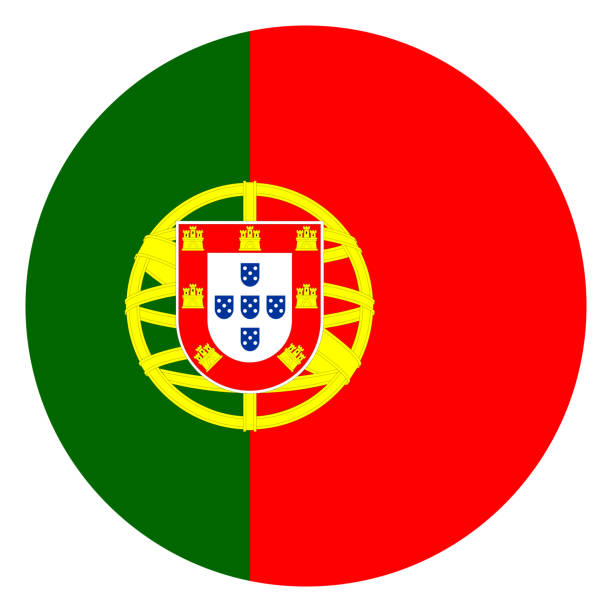
\includegraphics[width=0.19\textwidth]{Slides Principios de Economia/Figures/Magistral_07/M7.2.jpg}
    \hspace{15mm}
    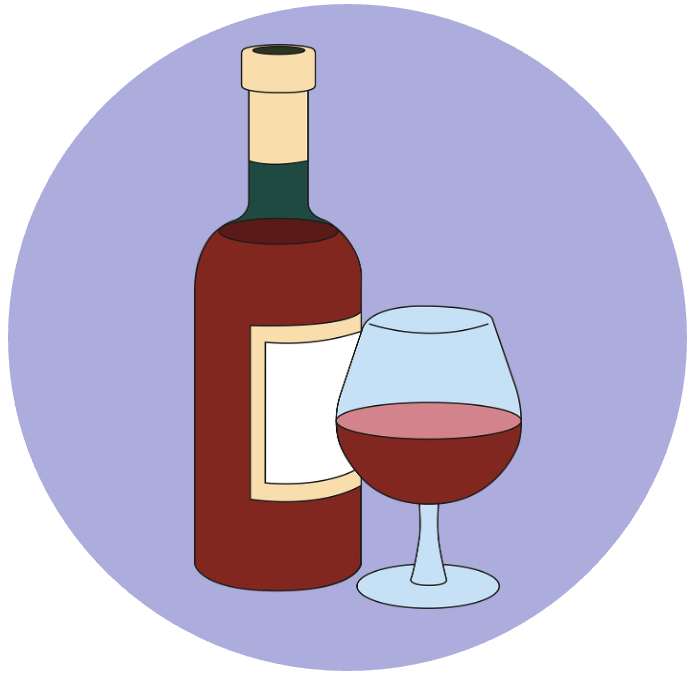
\includegraphics[width=0.18\textwidth]{Slides Principios de Economia/Figures/Magistral_07/M7.3.jpg}
    
\includegraphics[width=0.18\textwidth]{Slides Principios de Economia/Figures/Magistral_07/M7.4.jpg}
\end{figure}

\begin{itemize}
    \item 2 países: Inglaterra y Portugal\vspace{1.5mm}
    \item Dos productos: vino y telas\vspace{1.5mm}
    \item Portugal tiene la ventaja absoluta en ambos. 
        \begin{itemize}
        \item Inglaterra puede producirlos, pero Portugal tiene condiciones favorables tanto para producir uvas (para hacer el vino), como para criar ovejas (que dan la lana para las telas)\vspace{1.5mm}
        \end{itemize} 
    \item Para Inglaterra es relativamente más difícil producir vino\vspace{1.5mm}
    \item Inglaterra tendrá ventaja comparativa en tela y exportará a Portugal
\end{itemize} 
\end{frame}

\begin{frame}
\frametitle{Un modelo Ricardiano simple}
\begin{itemize}
    \item Supongamos que en Portugal (P) e Inglaterra (I) los bienes se producen sólo con trabajo (L). Los trabajadores de cada país son:
            \begin{equation*}
                \begin{aligned}
                L_P=25 \, \hspace{10mm} &\, L_I=100
                \end{aligned}
            \end{equation*}
    \item ¿Cúanto puede producir cada trabajador? \vspace{2mm}
        \begin{center}
            \begin{tabular}{|c|c|c|} \hline
            \rowcolor{blue!20}
                & Portugal & Inglaterra \\ \hline
                Vino por trabajador   & 4 & 1 \\ \hline
                Tela por trabajador   & 2 & 1 \\ \hline     
            \end{tabular}
        \end{center}
    \vspace{2mm}
    \item La productividad marginal del trabajo ($PMg$) entonces es: 
            \begin{equation*}
                \begin{aligned}
                    PMgL_V^{P} = 4 \, \hspace{10mm} &\, PMgL_T^{P} = 2 \\
                    PMgL_V^{I} = 1 \, \hspace{10mm}&\, PMgL_T^{I} = 1
                \end{aligned}
            \end{equation*}
       \vspace{-4mm}
     \item ¿Cuáles son las posibilidades de producción?    
    \end{itemize} 
\end{frame}


\begin{frame}{Frontera de Posibilidades de Producción}
    \begin{itemize}
        \item En ausencia de comercio, ¿qué cantidades de vino y tela producirían ambos países? 
        \vspace{2mm}
        \item Dada la cantidad de trabajadores y las productividades, podemos calcular cuánto produce un país si dedica todo su trabajo a un bien o a otro, o a una combinación de ambos.
    \end{itemize}
    \vspace{4mm}
    \begin{boxB}
        \centering
        La \textbf{frontera de posibilidades de producción (FPP)} muestra las combinaciones de bienes que un país puede producir con sus recursos y tecnología dados.
    \end{boxB}
\end{frame}

\begin{frame}
\frametitle{Portugal}

\begin{figure}[h]
    \centering
    \begin{tikzpicture}

        % Ejes
        \draw[thick,->] (0,0) -- (7,0) node[right] {$Q_{V}^{P}$};
        \draw[thick,->] (0,0) -- (0,6.5) node[left] {$Q_{T}^{P}$};

        % Línea de transformación
        \only<2->{
        \node[left] at (0,3) {\small $PMgL_T \cdot 25 = 50$};
        \fill (0,3) circle (2pt);
        }

        % Etiquetas en los ejes
        \only<3->{
        \node[below] at (5,0) {\small $PMgL_V \cdot  25 = 100$};
        \fill (5,0) circle (2pt);
        }
        \only<4->{
        \draw[thick, blue] (0,3) -- (5,0);
        
        % Flecha que indica la FPP
        \draw[->, thick, blue] (1,2.5) -- (1.5,2.8) node[above right] {FPP};
        }
        
        % Puntos
        \only<5->{
        \fill (2.5,1.5) circle (2pt);
        \fill (3.5,0.9) circle (2pt);

        % Delta etiquetas
        \draw[thin] (2.5,0.9) -- (3.5,0.9) node[midway,below] {\small $\Delta Q_{V}^{P}$};
        \draw[thin] (2.5,1.5) -- (2.5,0.9) node[midway,left] {\small $\Delta Q_{T}^{P}$};
        }
    \end{tikzpicture}
\end{figure}

\end{frame}

\begin{frame}{Portugal}
    \begin{itemize}
        \item La pendiente de la FPP nos indica el costo de oportunidad de producir una unidad adicional del bien que está en el eje X. \vspace{2mm}
        \item Si Portugal deja de producir 2 metros de tela, aumenta en 4 botellas la producción de vino.\vspace{2mm}
        \item Entonces el costo de oportunidad de producir una botella de vino extra para Portugal de $2/4 = 0,5$ metros de tela:\vspace{2mm}
        \[ \text{Pendiente} = \frac{\Delta Y}{\Delta X} = \frac{\Delta Q^{P}_T}{\Delta Q^{P}_V} = \frac{PMgL_T^{P}}{PMgL_V^{P}} = \frac{2}{4} = 0,5 \]
    \end{itemize}
\end{frame}

\begin{frame}
\frametitle{Eligiendo en Portugal}

\begin{figure}[h]
    \centering
    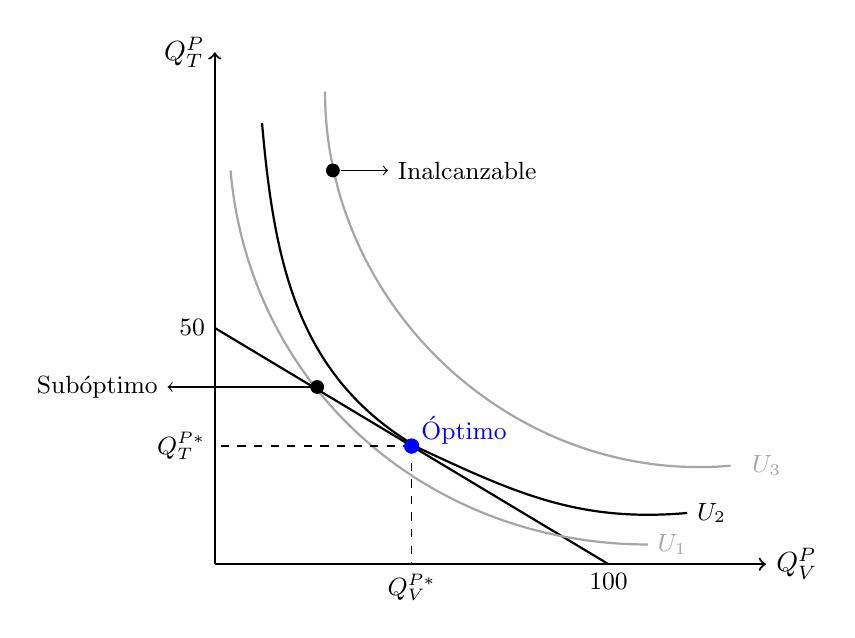
\begin{tikzpicture}

        % Ejes
        \draw[thick,->] (0,0) -- (7,0) node[right] {$Q_{V}^{P}$};
        \draw[thick,->] (0,0) -- (0,6.5) node[left] {$Q_{T}^{P}$};

        \node[below] at (5,0) {\small $100$};
        \node[left] at (0,3) {\small $50$};
        
        \draw[thick] (0,3) -- (5,0);

        \draw [thick, gray!70] (0.2,5) to [out=275,in=180] (5.5,0.25);
        \node [right, gray!70] at (5.5,0.25) {\small $U_1$};
        \draw [thick, black] (0.6,5.6) to [out=275,in=150] (2.6,1.47) to [out=335,in=185] (6,0.65);
        \node [right, black] at (6,0.65) {\small $U_2$};
        \draw [thick, gray!70] (1.4,6) to [out=270,in=185] (6.55,1.25);
        \node [right, gray!70] at (6.7,1.25) {\small $U_3$};

        % Lineas punteadas
        \draw[thin, dashed] (2.5,1.5) --  (0,1.5); \node[left] at (0,1.5) {\small $Q_{T}^{P*}$};
        \draw[thin, dashed] (2.5,1.5) -- (2.5,0); \node[below] at (2.5,0) {\small $Q_{V}^{P*}$};

         % Puntos
        \draw[fill, blue] (2.5,1.5) circle [radius =0.09];
        \node [right, blue] at (2.5,1.7) {\small Óptimo};

        \fill (1.3,2.25) circle (2.5pt);
        \draw[->, black] (1.225,2.25) -- (-0.6,2.25);
        \node[left] at (-0.6,2.25) {\small Subóptimo};

        \fill (1.5,5) circle (2.5pt);
        \draw[->, black] (1.6,5) -- (2.2,5);
        \node[right] at (2.2,5) {\small Inalcanzable};

    \end{tikzpicture}
\end{figure}

\end{frame}

\begin{frame}
\frametitle{Inglaterra}
\begin{figure}[h]
    \centering
    \begin{tikzpicture}

        % Ejes
        \draw[thick,->] (0,0) -- (7,0) node[right] {$Q_{V}^{I}$};
        \draw[thick,->] (0,0) -- (0,6.5) node[left] {$Q_{T}^{I}$};

        % Línea de transformación
        \node[left] at (0,5) {\small $PMgL_T \cdot 100 = 100$};
        \fill (0,5) circle (2pt);

        % Etiquetas en los ejes
        \node[below] at (5,0) {\small $PMgL_V \cdot  25 = 100$};
        \fill (5,0) circle (2pt);
        
        \draw[thick, blue] (0,5) -- (5,0);
        
        % Flecha que indica la FPP
        \draw[->, thick, blue] (1.8,3.3) -- (2.4,3.6) node[above right] {FPP};
        
        % Puntos
        \fill (2.5,2.5) circle (2pt);
        \fill (3.5,1.5) circle (2pt);

        % Delta etiquetas
        \draw[thin] (2.5,1.5) -- (3.5,1.5) node[midway,below] {\small $\Delta Q_{V}^{I}$};
        \draw[thin] (2.5,2.5) -- (2.5,1.5) node[midway,left] {\small $\Delta Q_{T}^{I}$};

    \end{tikzpicture}
\end{figure}
\end{frame}

\begin{frame}
\frametitle{Eligiendo en Inglaterra}
\begin{figure}[h]
    \centering
    \begin{tikzpicture}

        % Ejes
        \draw[thick,->] (0,0) -- (7,0) node[right] {$Q_{V}^{I}$};
        \draw[thick,->] (0,0) -- (0,6.5) node[left] {$Q_{T}^{I}$};

        \node[left] at (0,5) {\small $100$};
        \node[below] at (5,0) {\small $100$};
        
        \draw[thick, black] (0,5) -- (5,0);
        
        \fill (2.5,2.5) circle (2.5pt);

        \draw [thick, black] (1.2,5.7) to [out=270,in=180] (6,1.08);
        \node [right, black] at (6.1,1.1) {\small $U$};

        % Lineas punteadas
        \draw[thin, dashed] (2.5,2.5) --  (0,2.5); \node[left] at (0,2.5) {\small $Q_{T}^{I*}$};
        \draw[thin, dashed] (2.5,2.5) -- (2.5,0); \node[below] at (2.5,0) {\small $Q_{V}^{I*}$};

    \end{tikzpicture}
\end{figure}
\end{frame}

\begin{frame}
\frametitle{Ventaja comparativa}
\begin{itemize}
    \item El costo de oportunidad varía entre los distintos países\vspace{2mm}
        \begin{itemize}
        \item El costo de oportunidad de Portugal de producir una botella vino es igual a $2/4 =0,5$ metros de tela (o análogamente, su costo de oportunidad de producir un metro de tela es $4/2 =2$ botellas de vino).        \vspace{2mm}
        \item El costo de oportunidad de Inglaterra de producir una botella vino es igual a $1/1 =1$ metros de tela (o análogamente, su costo de oportunidad de producir un metro de tela es $1/1 =1$ botella de vino). 
        \end{itemize}
    \item Inglaterra tiene una ventaja comparativa en producir tela:
     \[ \begin{array}{c}
    \text{Costo de op. tela} \\ \text{Inglaterra}
    \end{array}= 1 \hspace{2mm} < \begin{array}{c}
    \hspace{2mm} \text{Costo de op. tela} \\ \text{Portugal}
    \end{array} = 2\] 
    \item Portugal tiene una ventaja comparativa en producir vino 
     \[ \begin{array}{c}
    \text{Costo de op. vino} \\ \text{Portugal}
    \end{array}= 0,5 \hspace{2mm} < \begin{array}{c}
    \hspace{2mm} \text{Costo de op. vino} \\ \text{Inglaterra}
    \end{array} = 1\] 
\end{itemize}
\end{frame}

\begin{frame}
\frametitle{Mercado y comercio}
\begin{itemize}
    \item Permitiendo que los países comercien, cada uno se especializará en el bien en el que tiene \textbf{ventaja comparativa}. \vspace{4mm}
    \item De esta manera, cada uno exportará la producción sobrante al otro país: Portugal exportará vino e Inglaterra exportará tela. 
\end{itemize}
\end{frame}

\begin{frame}
\frametitle{La producción de Portugal}
\begin{figure}[h]
    \centering
    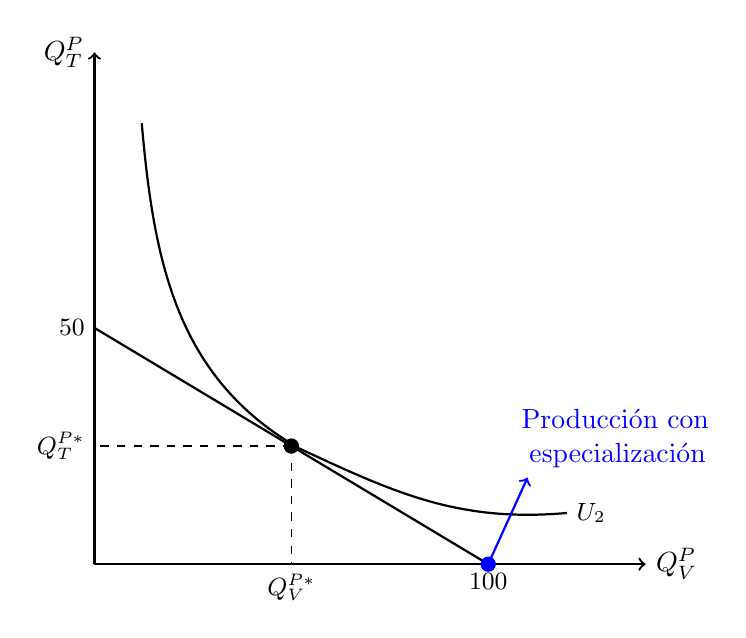
\begin{tikzpicture}

        % Ejes
        \draw[thick,->] (0,0) -- (7,0) node[right] {$Q_{V}^{P}$};
        \draw[thick,->] (0,0) -- (0,6.5) node[left] {$Q_{T}^{P}$};

        \node[below] at (5,0) {\small $100$};
        \node[left] at (0,3) {\small $50$};
        
        \draw[thick] (0,3) -- (5,0);

        \draw [thick, black] (0.6,5.6) to [out=275,in=150] (2.6,1.47) to [out=335,in=185] (6,0.65);
        \node [right, black] at (6,0.65) {\small $U_2$};

        % Lineas punteadas
        \draw[thin, dashed] (2.5,1.5) --  (0,1.5); \node[left] at (0,1.5) {\small $Q_{T}^{P*}$};
        \draw[thin, dashed] (2.5,1.5) -- (2.5,0); \node[below] at (2.5,0) {\small $Q_{V}^{P*}$};

         % Puntos
        \draw[fill, black] (2.5,1.5) circle [radius =0.09];

        \draw[fill, Blue] (5,0) circle [radius =0.09];
        \draw[->, thick, Blue] (5,0) -- (5.5,1.1);
        \node[above right, Blue] at (5.3,1.6) {Producción con};
        \node[above right, Blue] at (5.4,1.1) {especialización};

    \end{tikzpicture}
\end{figure}

\end{frame}

\begin{frame}{Portugal cuando comercia}
    \begin{itemize}
        \item Esto nos dice que los precios internos van a ser distintos (pensemos en términos de un trueque!)
        \item Ahora que Portugal se especializa tiene dos opciones:
        \begin{enumerate}
            \item Sacrificar 1 botella de vino para producir medio metro de tela (costo de oportunidad propio)
            \item Venderle a Inglaterra 1 botella de vino pidiéndole a cambio hasta un 1 metro de tela (que es lo que sacrificaría Inglaterra si quiere esa botella).
        \end{enumerate}
        \item Inglaterra está en la misma, especializándose en la tela:
        \begin{enumerate}
            \item Sacrificar 1 metro de tela para producir 1 botella de vino
            \item Venderle a Portugal 1 metro de tela, pidiéndole a cambio como mínimo 1 botella de vino pero como máximo 2 botellas (que es lo que sacrificaría Portugal si quiere ese metro de tela).
        \end{enumerate}
        \item Esto es exactamente lo mismo que pensar que los precios del bien que no produzco son menores en el otro país.
        \item Si esto sucede, la FPP de ambos países pivotea hacia afuera. 
    \end{itemize}
\end{frame}

\begin{frame}
\frametitle{Portugal cuando comercia}
\begin{figure}[h]
    \centering
    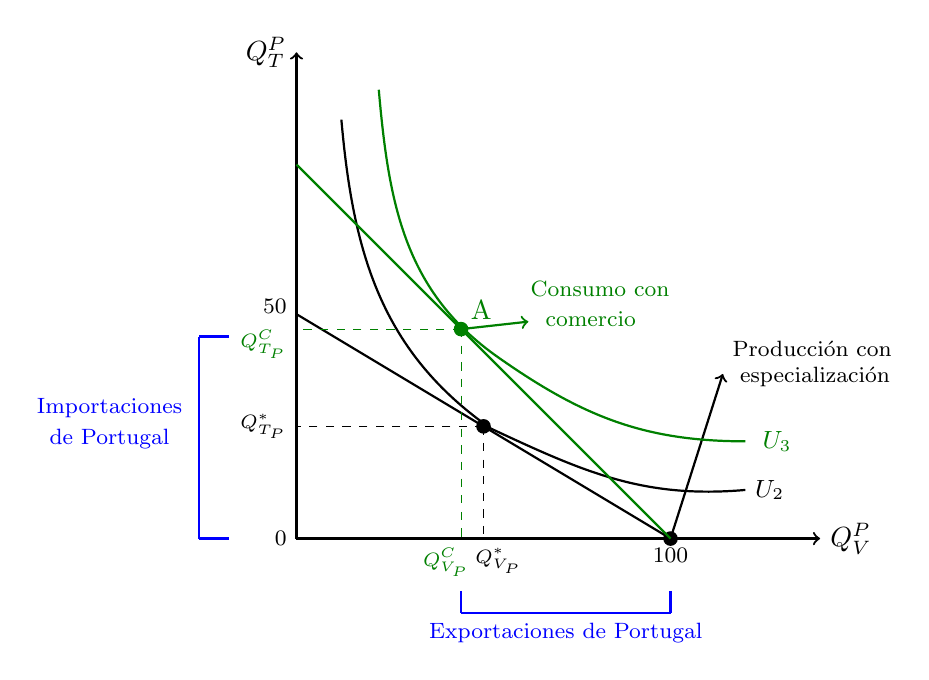
\begin{tikzpicture}[scale=0.95]

        % Ejes
        \draw[thick,->] (0,0) -- (7,0) node[right] {$Q_{V}^{P}$};
        \draw[thick,->] (0,0) -- (0,6.5) node[left] {$Q_{T}^{P}$};
        
        \draw[thick] (0,3) -- (5,0);
        \node[below] at (5,0) {\footnotesize $100$};
        \node[left] at (0,3.1) {\footnotesize $50$};
        \node[left] at (0,0) {\footnotesize $0$};

        \draw [thick, black] (0.6,5.6) to [out=275,in=145] (2.6,1.47) to [out=335,in=185] (6,0.65);
        \node [right, black] at (6,0.65) {\small $U_2$};

        % Lineas punteadas
        \draw[thin, dashed] (2.5,1.5) --  (0,1.5); \node[left] at (0,1.5) {\scriptsize $Q_{T_P}^{*}$};
        \draw[thin, dashed] (2.5,1.5) -- (2.5,0); \node[below] at (2.7,0) {\scriptsize $Q_{V_P}^{*}$};

         % Puntos
        \draw[fill, black] (2.5,1.5) circle [radius =0.09];

        \draw[fill] (5,0) circle [radius =0.09];
        \draw[->, thick] (5,0) -- (5.7,2.2);
        \node[above right] at (5.7,2.3) {\footnotesize Producción con};
        \node[above right] at (5.8,1.9) {\footnotesize especialización};

         % Con comercio
        \draw[thick, Green] (0,5) -- (5,0);
        \draw [thick, Green] (1.1,6) to [out=275,in=145] (2.7,2.42) to [out=325,in=180] (6,1.3);
        \node [right, Green] at (6.1,1.3)  {\small $U_3$};
        \draw[fill, Green] (2.2,2.8) circle [radius =0.09] node[above right] {A};
        \draw[thin, dashed, Green] (2.2,2.8) --  (0,2.8); \node[left, Green] at (0,2.6) {\scriptsize $Q_{T_P}^{C}$};
        \draw[thin, dashed, Green] (2.2,2.8) -- (2.2,0); \node[below, Green] at (2,0) {\scriptsize $Q_{V_P}^{C}$};
        \draw[->, thick, Green] (2.2,2.8) -- (3.1,2.9);
        \node[above right, Green] at (3,3.1) {\footnotesize Consumo con};
        \node[above right, Green] at (3.2,2.7) {\footnotesize comercio};

        % Expo Impo
        \draw[thick, Blue] (2.2,-1) --  (5,-1); 
        \draw[thick, Blue] (2.2,-0.7) --  (2.2,-1); 
        \draw[thick, Blue] (5,-0.7) --  (5,-1); 
        \node[below, Blue] at (3.6,-1) {\footnotesize Exportaciones de Portugal};

        \draw[thick, Blue] (-1.3,2.7) --  (-1.3,0); 
        \draw[thick, Blue] (-1.3,2.7) --  (-0.9,2.7); 
        \draw[thick, Blue] (-1.3,0) --  (-0.9,0); 
        \node[below, Blue] at (-2.5,2) {\footnotesize Importaciones};
        \node[below, Blue] at (-2.5,1.6) {\footnotesize de Portugal};

    \end{tikzpicture}
\end{figure}
\end{frame}

\begin{frame}{Inglaterra cuando comercia}
    \centering
    \begin{figure}[h]
        \centering
        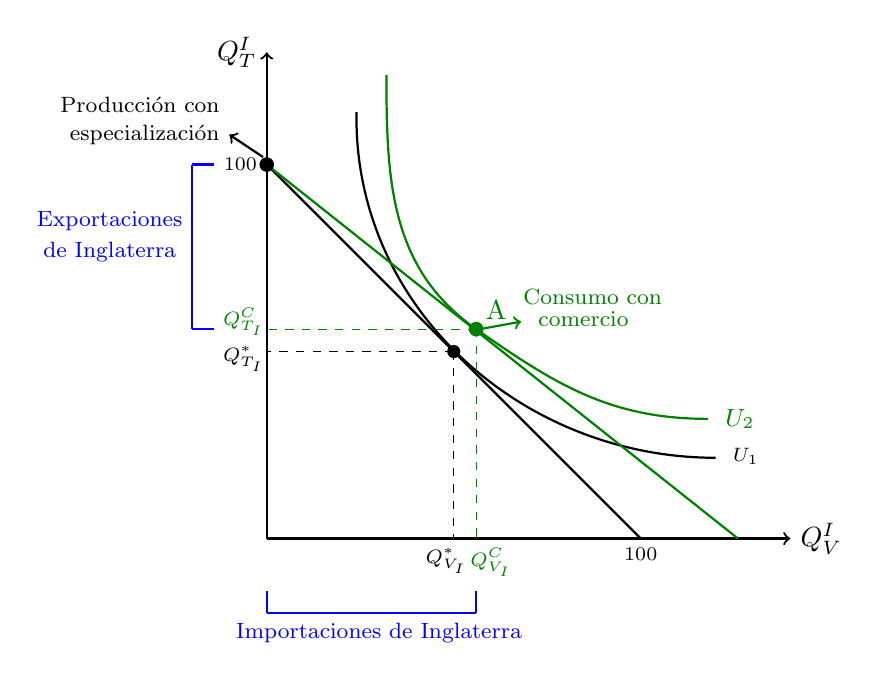
\begin{tikzpicture}[scale=0.95]

            % Ejes
            \draw[thick,->] (0,0) -- (7,0) node[right] {$Q_{V}^{I}$};
            \draw[thick,->] (0,0) -- (0,6.5) node[left] {$Q_{T}^{I}$};

            \node[left] at (0,5) {\scriptsize $100$};
            \node[below] at (5,0) {\scriptsize $100$};
            
            \draw[thick, black] (0,5) -- (5,0);
            
            \fill (2.5,2.5) circle (2.5pt);

            \draw [thick, black] (1.2,5.7) to [out=269,in=180] (6,1.08);
            \node [right, black] at (6.1,1.1) {\scriptsize $U_1$};

            % Lineas punteadas
            \draw[thin, dashed] (2.5,2.5) --  (0,2.5); \node[left] at (0.1,2.4) {\scriptsize $Q_{T_I}^{*}$};
            \draw[thin, dashed] (2.5,2.5) -- (2.5,0); \node[below] at (2.4,0) {\scriptsize $Q_{V_I}^{*}$};

            % Con comercio
            \draw[thick, Green] (0,5) -- (6.3,0);
            \draw [thick, Green] (1.6,6.2) to [out=270,in=145] (2.8,2.8) to [out=325,in=180] (5.9,1.6);
            \node [right, Green] at (6,1.6)  {\small $U_2$};
            \draw[fill, Green] (2.8,2.8) circle [radius =0.09] node[above right] {A};

            \draw[thin, dashed, Green] (2.8,2.8) --  (0,2.8); \node[left, Green] at (0.1,2.9) {\scriptsize $Q_{T_I}^{C}$};
            \draw[thin, dashed, Green] (2.8,2.8) -- (2.8,0); \node[below, Green] at (3,0) {\scriptsize $Q_{V_I}^{C}$};

            \draw[->, thick, Green] (2.85,2.8) -- (3.4,2.9);
            \node[above right, Green] at (3.3,3) {\footnotesize Consumo con};
            \node[above right, Green] at (3.5,2.7) {\footnotesize comercio};

            \draw[fill] (0,5) circle [radius =0.09];
            \draw[->, thick] (-0.05,5.1) -- (-0.5,5.4);
            \node[ left] at (-0.5,5.8) {\footnotesize Producción con};
            \node[ left] at (-0.5,5.4) {\footnotesize especialización};

            % Expo Impo
            \draw[thick, Blue] (0,-1) --  (2.8,-1); 
            \draw[thick, Blue] (0,-0.7) --  (0,-1); 
            \draw[thick, Blue] (2.8,-0.7) --  (2.8,-1); 
            \node[below, Blue] at (1.5,-1) {\footnotesize Importaciones de Inglaterra};

            \draw[thick, Blue] (-1,5) --  (-1,2.8); 
            \draw[thick, Blue] (-1,2.8) --  (-0.7,2.8); 
            \draw[thick, Blue] (-1,5) --  (-0.7,5); 
            \node[below, Blue] at (-2.1,4.5) {\footnotesize Exportaciones};
            \node[below, Blue] at (-2.1,4.1) {\footnotesize de Inglaterra};

        \end{tikzpicture}
    \end{figure}
\end{frame}

\begin{frame}
    \frametitle{Conclusiones}
    \begin{itemize}
        \item Cuando dejamos que los países se especialicen y comercien, nos encontramos con que estarán en un escenario mejor en comparación con la situación en ausencia de comercio.
        \item No sabemos el precio al que se terminan comerciando los bienes porque queda indefinido. Aunque necesariamente estará entre la TMT de los dos países.
        \item La presencia de mercados logra algo notable: cooperación no intencionada entre extraños.
        \item El libre comercio ejemplifica un juego en el que todos los participantes pueden beneficiarse de un escenario en el que todos ganan, todos cooperan para alcanzar el beneficio máximo.
        \item La economía es la ciencia del "win-win".
    \end{itemize}
\end{frame}


\end{document}




%%%%%%%%%%%%%%%%%%%%%%%%%%%%%%%%%%%%%%%%%%%%%%%%%%%%%%%%%%%%%%%%%%%%%%%%%
\begin{frame}
\frametitle{Teoría de juegos}
\begin{itemize}
\item Estudia de manera formal y abstracta las decisiones óptimas que deben tomar diversos adversarios en conflicto.\vspace{4mm}
\item Es el estudio matemático de la toma de decisiones, del conflicto y la estrategia en situaciones sociales.\vspace{4mm}
\item Los jugadores toman decisiones que se consideran estratégicas\vspace{2mm}
    \begin{itemize}
        \item los jugadores son entes racionales (no necesariamente humanos)\vspace{2mm}
        \item los entes que participan en el juego actúan teniendo en cuenta las acciones que tomarían los demás
            \end{itemize}
\end{itemize}
\end{frame}


\begin{frame}
\frametitle{Elementos de un juego}
\begin{itemize}
\item \textbf{Los jugadores:} quién está interactuando con quién.\vspace{4mm}
\item \textbf{Las estrategias viables:} qué acciones están abiertas a los jugadores.\vspace{4mm}
\item \textbf{La información:} lo que cada jugador sabe al tomar su decisión.\vspace{4mm}
\item \textbf{Los beneficios:} cuáles serán los resultados para cada una de las posibles combinaciones de acciones.\vspace{4mm}
\end{itemize}
\end{frame}

\begin{frame}
\frametitle{Tipos de juegos}
\begin{itemize}
\item Juegos simultáneos: donde se toma una decisión one-shot.\vspace{4mm}
\item Juegos secuenciales: donde los jugadores toman sus decisiones de forma consecutiva.\vspace{4mm}
\item Juego de información perfecta: donde los individuos conocen las reglas del juego.\vspace{4mm}
\item  Juegos de información completa: donde los individuos conocen las movidas que hicieron los otros jugadores.\vspace{4mm}
\item  Juegos de información incompleta: donde los individuo no conocen la historia.
\end{itemize}
\end{frame}


%\begin{frame}
%\frametitle{Estudiando juegos}
%\begin{itemize}
%\item El término ``juegos'' refiere básicamente a modelos de interacción estratégica
%\begin{itemize}
%    \item Es decir, modelos donde las personas involucradas en una interacción social saben que sus acciones afectan a otros y viceversa
  
 %       \item En este contexto, una estrategia es una acción (o un curso de acción) que puede tomar una persona cuando es consciente de esta dependencia mutua de los resultados
   
%\end{itemize}

%\end{itemize}
%\end{frame}




\begin{frame}
\frametitle{23. Juegos simultáneos}
\begin{itemize}
\item En los juegos simultáneos, cada jugador decide su estrategia antes de conocer las decisiones de otros jugadores
\item Para analizar estos juegos, usamos la matriz o forma estratégica de un juego
\item La combinación de las estrategias elegidas por los jugadores determina la ganancia de cada jugador
\end{itemize}
\end{frame}


\begin{frame}
\frametitle{25. Dilema del prisionero}
\begin{itemize}
\item Dos sospechosos son arrestados y acusados de un delito
\item La policía no tiene evidencia suficiente para condenar a los sospechosos a menos que uno confiese
\item La policía encierra a los sospechosos en celdas separadas y les explica las consecuencias derivadas de las decisiones que formen
\end{itemize}
\end{frame}

\begin{frame}
\frametitle{26. Dilema de los prisioneros}
\begin{itemize}
\item Si ninguno confiesa, ambos serán condenados por un delito menor sentenciados a un mes de cárcel
\item Si ambos, confiesan serán sentenciados a seis meses de cárcel
\item Finalmente, si uno confiesa y el otro no, el que confiesa será puesto en libertad inmediatamente y el otro
será sentenciado a nueve meses en prisión, seis por el delito y tres más por obstrucción a la justicia
\end{itemize}
\end{frame}

\begin{frame}
\frametitle{27. Dilema de los prisioneros}
\begin{table}
     \begin{tabular}{cc|c|c|}
      & \multicolumn{1}{c}{} & \multicolumn{2}{c}{Preso $2$}\\
      & \multicolumn{1}{c}{} & \multicolumn{1}{c}{No confesar}  & \multicolumn{1}{c}{Confesar} \\\cline{3-4}
      \multirow{}{Preso $1$}  & No Confesar & $(-1,-1)$ & $(-9,0)$ \\\cline{3-4}
      & Confesar & $(0,-9)$ & $(-6,-6)$ \\\cline{3-4}
    \end{tabular}
  \end{table}
\end{frame}

\begin{frame}
\frametitle{28. Dilema de los prisioneros}
\begin{itemize}
\item Cada jugador cuenta con dos estrategias posibles: confesar y no confesar. 
\item Las ganancias de los dos jugadores cuando eligen un par concreto de estrategias aparecen en la casilla correspondiente de la matriz binaria. 
\item Por convención, la ganancia del llamado jugador-fila (Preso 1) es la primera ganancia, seguida, por la ganancia del jugador columna (Preso 2). 
\end{itemize}
\end{frame}

\begin{frame}
\frametitle{29. Dilema de los prisioneros}
\begin{itemize}
\item Por ejemplo, el preso 1 elige no confesar y el preso 2 elige confesar, el preso 1 recibe una ganancia de -9 (que representa nueve meses en prisión) y el preso 2 recibe una ganancia de 0 (que representa la inmediata puesta en libertad).
\item La representación en forma normal de un juego especifica: 
\begin{enumerate}
\item [1] los jugadores en el juego,
\item [2] las estrategias de que dispone cada jugador, y 
\item [3] la ganancia de cada jugador en cada combinación posible de estrategias.
\end{enumerate}
\end{itemize}
\end{frame}







$$$$$$$$$$$$$$
\begin{frame}
\frametitle{22. Teoría de juegos y estrategia competitiva}
\begin{block}{Equilibrio de Nash}
Un equilibrio de Nash es un par de estrategias, una para cada jugador, en las que cada estrategia es la mejor respuesta dado lo que hace el otro
\end{block}
\vspace{5mm}
En equilibrio, cada jugador está haciendo lo mejor que puede, dado lo que el otro jugador también lo está haciendo
\end{frame}
$$$$$$$$$$$$$$$$$$